\chapter{Smith-Hutton problem}
The Smith-Hutton problem is a two-dimensional steady convection-diffusion problem, represented in figure \ref{SHscheme}. The density is constant, and the velocity field is known.
\begin{figure}[h!]
	\centering
	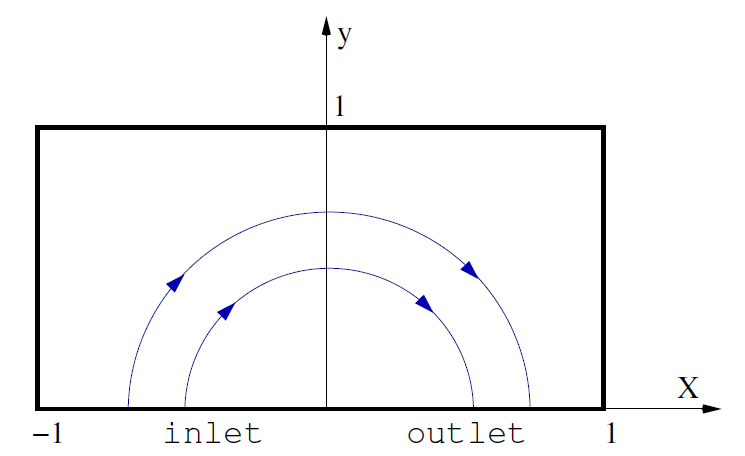
\includegraphics[scale=0.65]{SmithHutton/SmithHutton}
	\caption{General scheme of the Smith-Hutton problem}
	\label{SHscheme}
\end{figure}

The prescribed velocity field is given by:
\begin{equation}
u\left(x,y\right)=2y\left(1-x^{2}\right)
\end{equation}
\begin{equation}
v\left(x,y\right)=-2x\left(1-y^{2}\right)
\end{equation}
And the prescribed boundary conditions for the variable $\phi$ are:
\begin{equation}
\begin{aligned}
\phi &=1+\tanh\left(\alpha\left(2x+1\right)\right),&&y=0; x\in\left(-1,0\right) \left(inlet\right) \\
\frac{\partial\phi}{\partial y} &=0,&&x=0; y\in\left(-1,0\right) \left(outlet\right) \\
\phi &=1-\tanh\left(\alpha\right),&&\left(elsewhere\right)
\end{aligned}
\label{BoundCond}
\end{equation}
where $\alpha=10$.

\section{Discretization}
The spatial discretization is the one explained in section \ref{DiscretizationSH}, and the temporal scheme used is the implicit one, as explained in the same section.

\begin{table}[h]
	\centering
	\begin{tabular}{ |c|c|c|c| }
		\hline
		$N_{x}$ & $N_{y}$ & $\delta$ & Source term \\ \hline
		$200$ & $100$ & $10^{-9}$ & $0$ \\ \hline
	\end{tabular}
\caption{Numerical parameters of the Smith-Hutton problem}
\end{table}

\section{Boundary conditions}
To apply the boundary conditions to the problem, some modifications on the coefficients defined by equation \ref{DiscretizedEquGCDE} have to be done. The easiest one is for the points in the left, top and right sides of the domain, in which the value of $\phi$ is defined.

In the bottom it is necessary to distinguish between the inlet and the outlet. A similar approach to that of the left, top and right side is used to determine the coefficients of the points in the inlet. However, in the outlet the only condition is that the derivative of $\phi$ in the vertical direction is equal to zero. The following reasoning leads to:
\begin{equation}
\frac{\partial\phi}{\partial y}\approx\frac{\phi_{N}-\phi_{P}}{\Delta y}=0
\end{equation}
\begin{equation}
\phi_{P}=\phi_{N}
\end{equation}
The implementation of the boundary conditions in the problem is done with the discretization coefficients listed in table \ref{BoundaryCondSH}.
\begin{table}[h]
	\centering
	\begin{tabular}{ |c|c|c|c| }
		\hline
		Coefficients & Left, top and right & Inlet (bottom) & Outlet (bottom) \\ \hline
		$a_{E}$ & $0$ & $0$ & $0$ \\ \hline
		$a_{W}$ & $0$ & $0$ & $0$ \\ \hline
		$a_{N}$ & $0$ & $0$ & $1$ \\ \hline
		$a_{S}$ & $0$ & $0$ & $0$ \\ \hline
		$a_{P}$ & $1$ & $1$ & $1$ \\ \hline
		$b_{P}$ & $1-\tanh\left(\alpha\right)$ & $1+\tanh\left(\alpha\left(2x+1\right)\right)$ & $0$ \\ \hline
	\end{tabular}
\caption{Discretization coefficients of the boundary points}
\label{BoundaryCondSH}
\end{table}


\section{Algorithm}
The algorithm of resolution is very similar to that used in the four materials problem. The main difference is that in the Smith-Hutton problem the resolution ends when the variable $\phi$ reaches a steady state. The schematic algorithm of resolution is displayed below:
\begin{figure}[h!]
	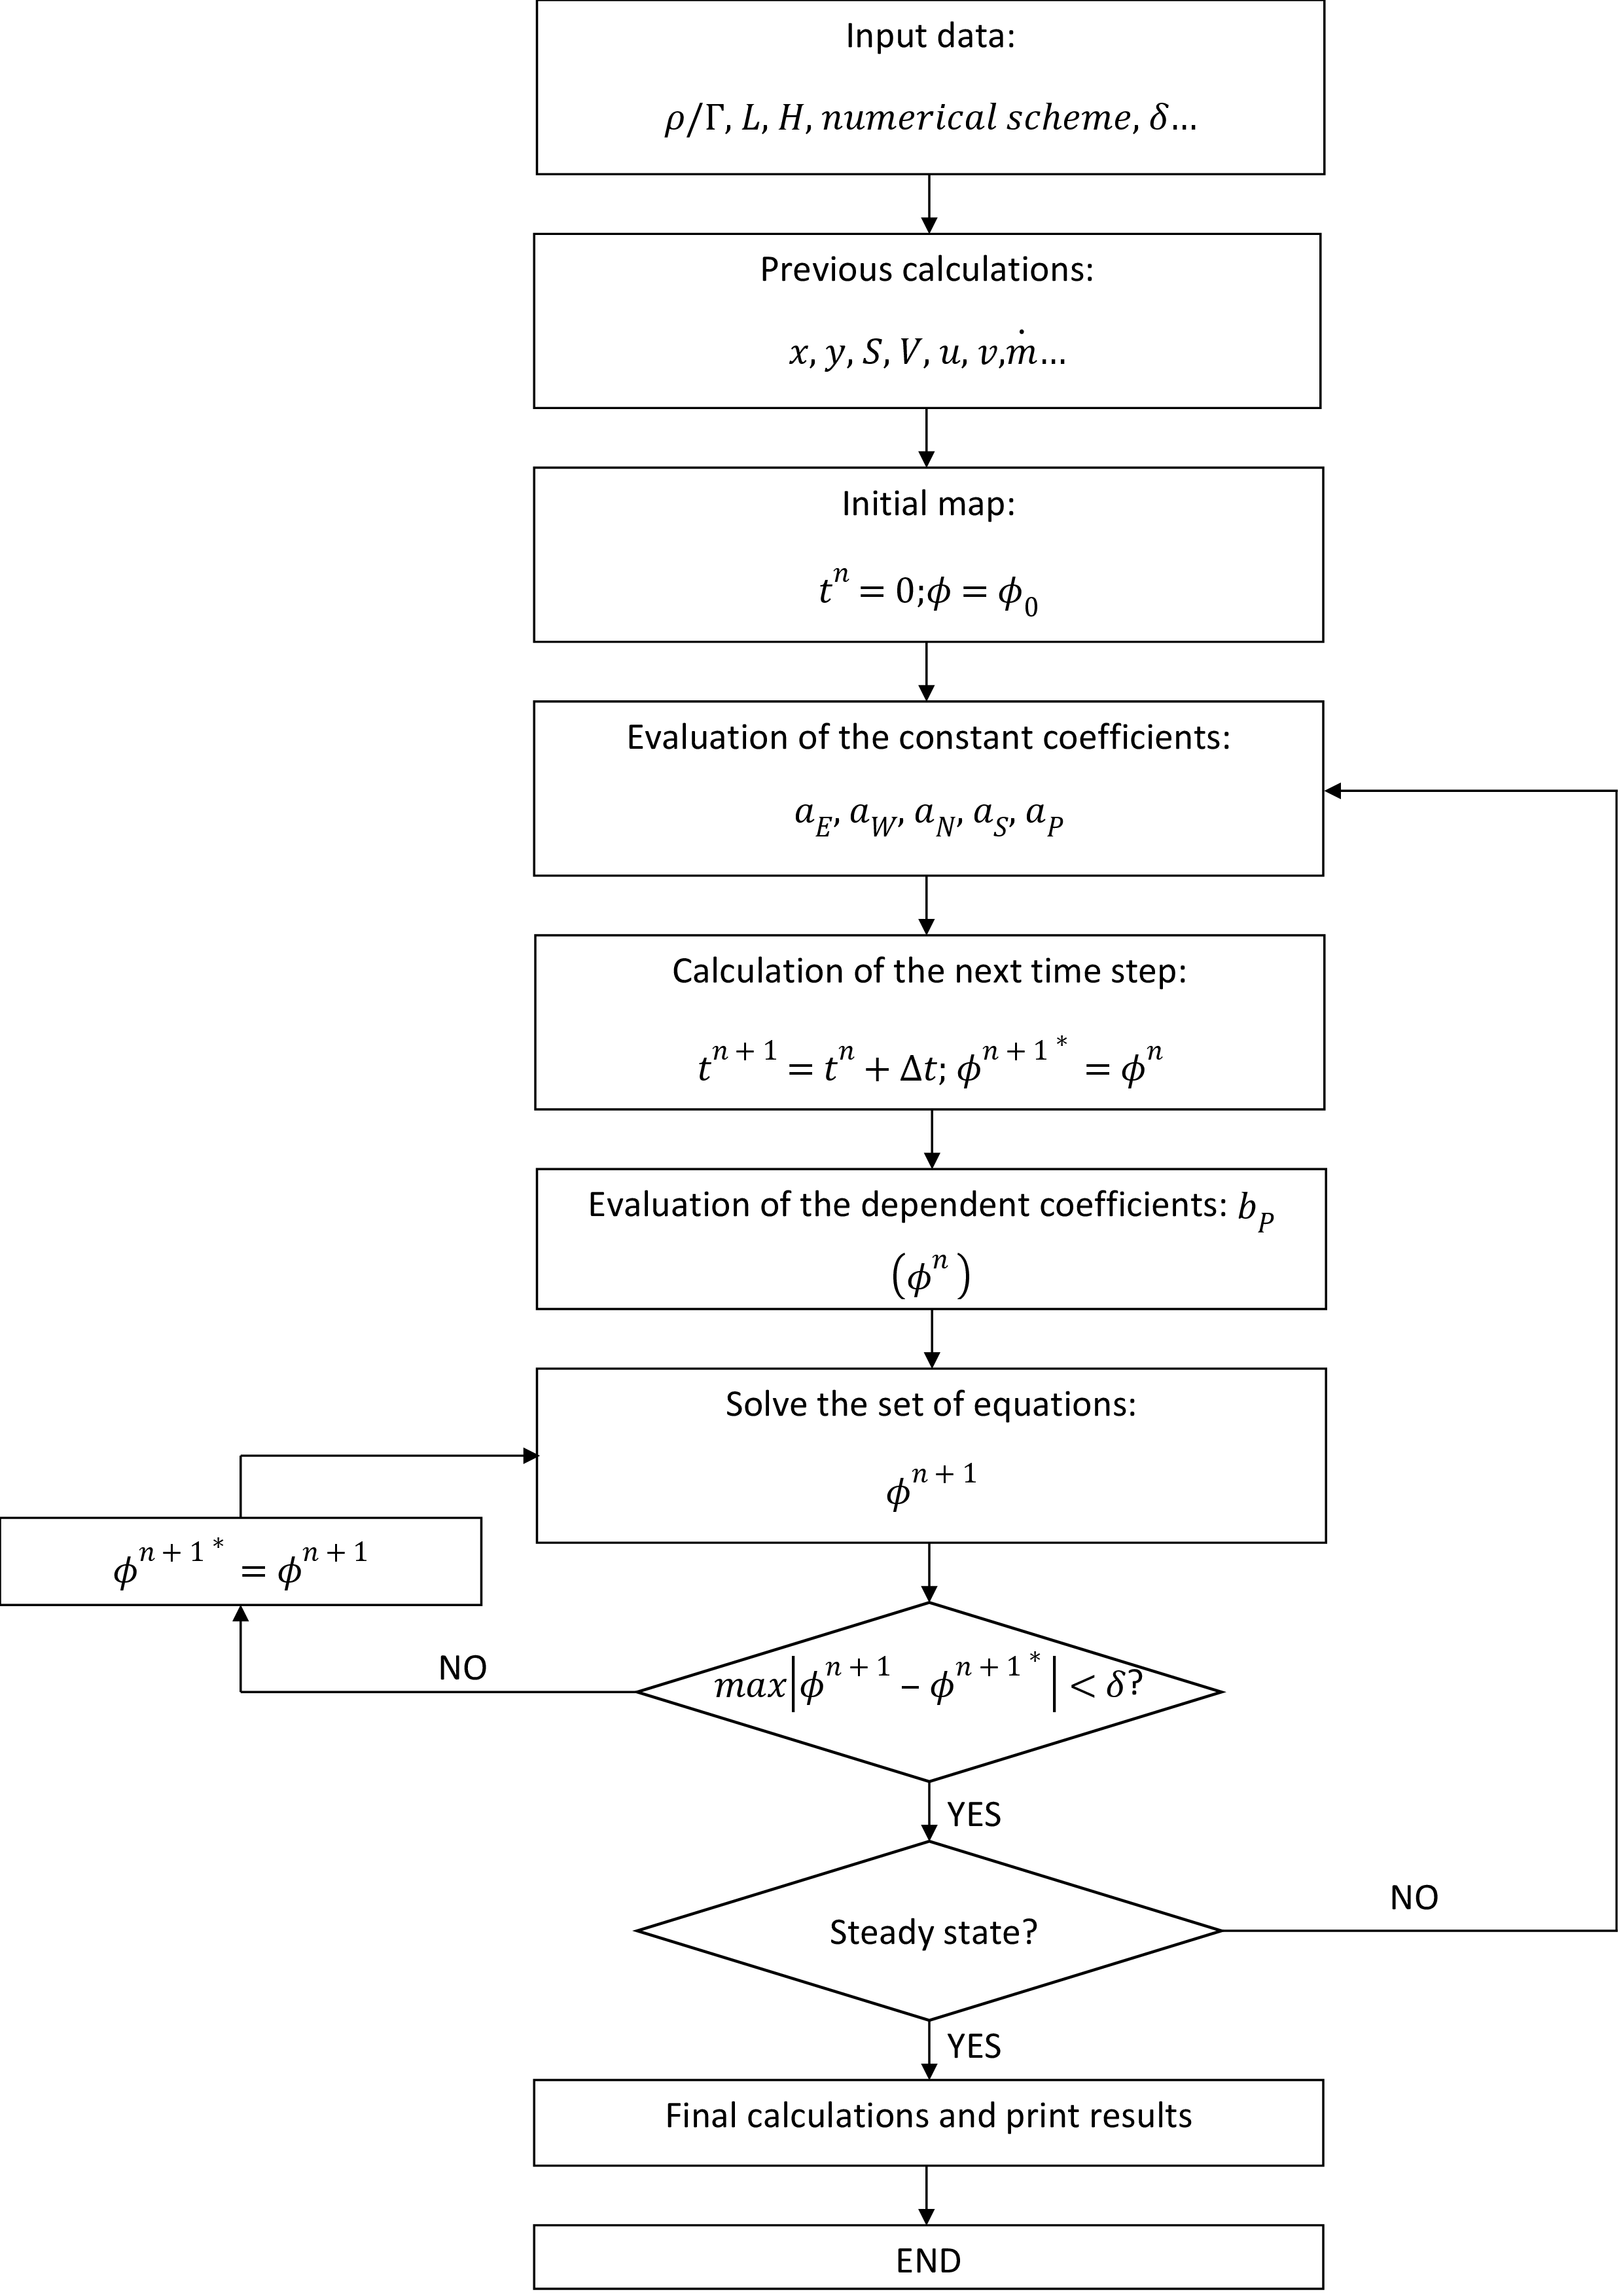
\includegraphics[scale=0.17]{SmithHutton/algorithm}
\end{figure}

\section{Results}
Since the velocity and the dimensions are constant, the parameter $\rho/\Gamma$ is somehow equivalent to the Péclet number. In order to study the results in different flows, the simulation has been run for three different values of $\rho/\Gamma$: $10$, $10^{3}$ and $10^{6}$.

To verify the accuracy of the calculations and the influence of the numerical scheme, the results have to be compared with some reference values. The following figures present the distribution of the variable $\phi$ in the outlet for all the schemes used and compare them with the benchmark values.

In figure \ref{ResSH10}, when the Péclet number is low, all the methods produce similar results, and there is almost no error compared to the reference values. However, as the Péclet number increases, the error also increases. As it can be seen in figures \ref{ResSH1000} and \ref{ResSH1000000}, the reference solution displays a sharper distribution than the one obtained in the calculations. The influence of the numerical scheme used is also present in the case of $\rho/\Gamma=10^{3}$, when the schemes show slightly different results.

\begin{figure}[h]
	\centering
	% GNUPLOT: LaTeX picture with Postscript
\begingroup
  \makeatletter
  \providecommand\color[2][]{%
    \GenericError{(gnuplot) \space\space\space\@spaces}{%
      Package color not loaded in conjunction with
      terminal option `colourtext'%
    }{See the gnuplot documentation for explanation.%
    }{Either use 'blacktext' in gnuplot or load the package
      color.sty in LaTeX.}%
    \renewcommand\color[2][]{}%
  }%
  \providecommand\includegraphics[2][]{%
    \GenericError{(gnuplot) \space\space\space\@spaces}{%
      Package graphicx or graphics not loaded%
    }{See the gnuplot documentation for explanation.%
    }{The gnuplot epslatex terminal needs graphicx.sty or graphics.sty.}%
    \renewcommand\includegraphics[2][]{}%
  }%
  \providecommand\rotatebox[2]{#2}%
  \@ifundefined{ifGPcolor}{%
    \newif\ifGPcolor
    \GPcolortrue
  }{}%
  \@ifundefined{ifGPblacktext}{%
    \newif\ifGPblacktext
    \GPblacktexttrue
  }{}%
  % define a \g@addto@macro without @ in the name:
  \let\gplgaddtomacro\g@addto@macro
  % define empty templates for all commands taking text:
  \gdef\gplbacktext{}%
  \gdef\gplfronttext{}%
  \makeatother
  \ifGPblacktext
    % no textcolor at all
    \def\colorrgb#1{}%
    \def\colorgray#1{}%
  \else
    % gray or color?
    \ifGPcolor
      \def\colorrgb#1{\color[rgb]{#1}}%
      \def\colorgray#1{\color[gray]{#1}}%
      \expandafter\def\csname LTw\endcsname{\color{white}}%
      \expandafter\def\csname LTb\endcsname{\color{black}}%
      \expandafter\def\csname LTa\endcsname{\color{black}}%
      \expandafter\def\csname LT0\endcsname{\color[rgb]{1,0,0}}%
      \expandafter\def\csname LT1\endcsname{\color[rgb]{0,1,0}}%
      \expandafter\def\csname LT2\endcsname{\color[rgb]{0,0,1}}%
      \expandafter\def\csname LT3\endcsname{\color[rgb]{1,0,1}}%
      \expandafter\def\csname LT4\endcsname{\color[rgb]{0,1,1}}%
      \expandafter\def\csname LT5\endcsname{\color[rgb]{1,1,0}}%
      \expandafter\def\csname LT6\endcsname{\color[rgb]{0,0,0}}%
      \expandafter\def\csname LT7\endcsname{\color[rgb]{1,0.3,0}}%
      \expandafter\def\csname LT8\endcsname{\color[rgb]{0.5,0.5,0.5}}%
    \else
      % gray
      \def\colorrgb#1{\color{black}}%
      \def\colorgray#1{\color[gray]{#1}}%
      \expandafter\def\csname LTw\endcsname{\color{white}}%
      \expandafter\def\csname LTb\endcsname{\color{black}}%
      \expandafter\def\csname LTa\endcsname{\color{black}}%
      \expandafter\def\csname LT0\endcsname{\color{black}}%
      \expandafter\def\csname LT1\endcsname{\color{black}}%
      \expandafter\def\csname LT2\endcsname{\color{black}}%
      \expandafter\def\csname LT3\endcsname{\color{black}}%
      \expandafter\def\csname LT4\endcsname{\color{black}}%
      \expandafter\def\csname LT5\endcsname{\color{black}}%
      \expandafter\def\csname LT6\endcsname{\color{black}}%
      \expandafter\def\csname LT7\endcsname{\color{black}}%
      \expandafter\def\csname LT8\endcsname{\color{black}}%
    \fi
  \fi
    \setlength{\unitlength}{0.0500bp}%
    \ifx\gptboxheight\undefined%
      \newlength{\gptboxheight}%
      \newlength{\gptboxwidth}%
      \newsavebox{\gptboxtext}%
    \fi%
    \setlength{\fboxrule}{0.5pt}%
    \setlength{\fboxsep}{1pt}%
\begin{picture}(7200.00,5040.00)%
    \gplgaddtomacro\gplbacktext{%
      \csname LTb\endcsname%
      \put(814,704){\makebox(0,0)[r]{\strut{}$0$}}%
      \put(814,1111){\makebox(0,0)[r]{\strut{}$0.2$}}%
      \put(814,1518){\makebox(0,0)[r]{\strut{}$0.4$}}%
      \put(814,1925){\makebox(0,0)[r]{\strut{}$0.6$}}%
      \put(814,2332){\makebox(0,0)[r]{\strut{}$0.8$}}%
      \put(814,2740){\makebox(0,0)[r]{\strut{}$1$}}%
      \put(814,3147){\makebox(0,0)[r]{\strut{}$1.2$}}%
      \put(814,3554){\makebox(0,0)[r]{\strut{}$1.4$}}%
      \put(814,3961){\makebox(0,0)[r]{\strut{}$1.6$}}%
      \put(814,4368){\makebox(0,0)[r]{\strut{}$1.8$}}%
      \put(814,4775){\makebox(0,0)[r]{\strut{}$2$}}%
      \put(946,484){\makebox(0,0){\strut{}$0$}}%
      \put(2117,484){\makebox(0,0){\strut{}$0.2$}}%
      \put(3289,484){\makebox(0,0){\strut{}$0.4$}}%
      \put(4460,484){\makebox(0,0){\strut{}$0.6$}}%
      \put(5632,484){\makebox(0,0){\strut{}$0.8$}}%
      \put(6803,484){\makebox(0,0){\strut{}$1$}}%
    }%
    \gplgaddtomacro\gplfronttext{%
      \csname LTb\endcsname%
      \put(176,2739){\rotatebox{-270}{\makebox(0,0){\strut{}$\phi$}}}%
      \put(3874,154){\makebox(0,0){\strut{}x-position}}%
      \csname LTb\endcsname%
      \put(5816,4602){\makebox(0,0)[r]{\strut{}Reference}}%
      \csname LTb\endcsname%
      \put(5816,4382){\makebox(0,0)[r]{\strut{}CDS}}%
      \csname LTb\endcsname%
      \put(5816,4162){\makebox(0,0)[r]{\strut{}UDS}}%
      \csname LTb\endcsname%
      \put(5816,3942){\makebox(0,0)[r]{\strut{}HDS}}%
      \csname LTb\endcsname%
      \put(5816,3722){\makebox(0,0)[r]{\strut{}PLDS}}%
      \csname LTb\endcsname%
      \put(5816,3502){\makebox(0,0)[r]{\strut{}EDS}}%
    }%
    \gplbacktext
    \put(0,0){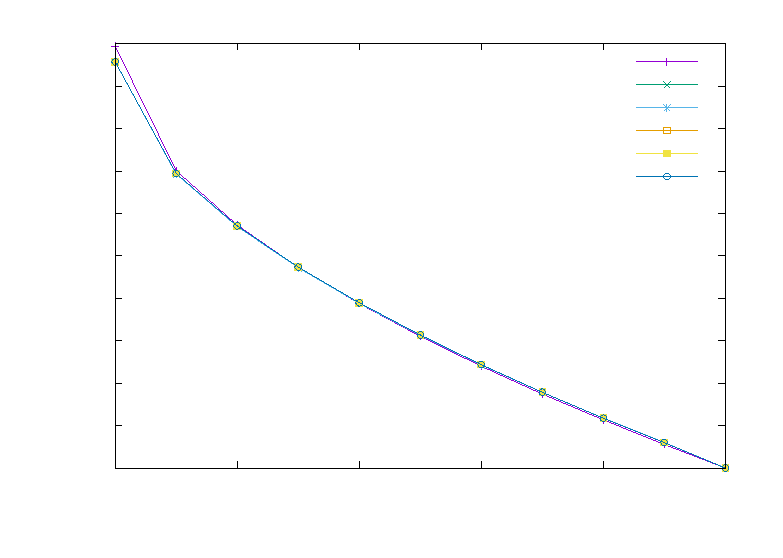
\includegraphics{SmithHutton/10}}%
    \gplfronttext
  \end{picture}%
\endgroup

	\caption{Distribution of $\phi$ at the output for $\rho/\Gamma=10$}
	\label{ResSH10}
\end{figure}
\begin{figure}[h]
	\centering
	% GNUPLOT: LaTeX picture with Postscript
\begingroup
  \makeatletter
  \providecommand\color[2][]{%
    \GenericError{(gnuplot) \space\space\space\@spaces}{%
      Package color not loaded in conjunction with
      terminal option `colourtext'%
    }{See the gnuplot documentation for explanation.%
    }{Either use 'blacktext' in gnuplot or load the package
      color.sty in LaTeX.}%
    \renewcommand\color[2][]{}%
  }%
  \providecommand\includegraphics[2][]{%
    \GenericError{(gnuplot) \space\space\space\@spaces}{%
      Package graphicx or graphics not loaded%
    }{See the gnuplot documentation for explanation.%
    }{The gnuplot epslatex terminal needs graphicx.sty or graphics.sty.}%
    \renewcommand\includegraphics[2][]{}%
  }%
  \providecommand\rotatebox[2]{#2}%
  \@ifundefined{ifGPcolor}{%
    \newif\ifGPcolor
    \GPcolortrue
  }{}%
  \@ifundefined{ifGPblacktext}{%
    \newif\ifGPblacktext
    \GPblacktexttrue
  }{}%
  % define a \g@addto@macro without @ in the name:
  \let\gplgaddtomacro\g@addto@macro
  % define empty templates for all commands taking text:
  \gdef\gplbacktext{}%
  \gdef\gplfronttext{}%
  \makeatother
  \ifGPblacktext
    % no textcolor at all
    \def\colorrgb#1{}%
    \def\colorgray#1{}%
  \else
    % gray or color?
    \ifGPcolor
      \def\colorrgb#1{\color[rgb]{#1}}%
      \def\colorgray#1{\color[gray]{#1}}%
      \expandafter\def\csname LTw\endcsname{\color{white}}%
      \expandafter\def\csname LTb\endcsname{\color{black}}%
      \expandafter\def\csname LTa\endcsname{\color{black}}%
      \expandafter\def\csname LT0\endcsname{\color[rgb]{1,0,0}}%
      \expandafter\def\csname LT1\endcsname{\color[rgb]{0,1,0}}%
      \expandafter\def\csname LT2\endcsname{\color[rgb]{0,0,1}}%
      \expandafter\def\csname LT3\endcsname{\color[rgb]{1,0,1}}%
      \expandafter\def\csname LT4\endcsname{\color[rgb]{0,1,1}}%
      \expandafter\def\csname LT5\endcsname{\color[rgb]{1,1,0}}%
      \expandafter\def\csname LT6\endcsname{\color[rgb]{0,0,0}}%
      \expandafter\def\csname LT7\endcsname{\color[rgb]{1,0.3,0}}%
      \expandafter\def\csname LT8\endcsname{\color[rgb]{0.5,0.5,0.5}}%
    \else
      % gray
      \def\colorrgb#1{\color{black}}%
      \def\colorgray#1{\color[gray]{#1}}%
      \expandafter\def\csname LTw\endcsname{\color{white}}%
      \expandafter\def\csname LTb\endcsname{\color{black}}%
      \expandafter\def\csname LTa\endcsname{\color{black}}%
      \expandafter\def\csname LT0\endcsname{\color{black}}%
      \expandafter\def\csname LT1\endcsname{\color{black}}%
      \expandafter\def\csname LT2\endcsname{\color{black}}%
      \expandafter\def\csname LT3\endcsname{\color{black}}%
      \expandafter\def\csname LT4\endcsname{\color{black}}%
      \expandafter\def\csname LT5\endcsname{\color{black}}%
      \expandafter\def\csname LT6\endcsname{\color{black}}%
      \expandafter\def\csname LT7\endcsname{\color{black}}%
      \expandafter\def\csname LT8\endcsname{\color{black}}%
    \fi
  \fi
    \setlength{\unitlength}{0.0500bp}%
    \ifx\gptboxheight\undefined%
      \newlength{\gptboxheight}%
      \newlength{\gptboxwidth}%
      \newsavebox{\gptboxtext}%
    \fi%
    \setlength{\fboxrule}{0.5pt}%
    \setlength{\fboxsep}{1pt}%
\begin{picture}(7200.00,5040.00)%
    \gplgaddtomacro\gplbacktext{%
      \csname LTb\endcsname%
      \put(814,704){\makebox(0,0)[r]{\strut{}$0$}}%
      \put(814,1722){\makebox(0,0)[r]{\strut{}$0.5$}}%
      \put(814,2740){\makebox(0,0)[r]{\strut{}$1$}}%
      \put(814,3757){\makebox(0,0)[r]{\strut{}$1.5$}}%
      \put(814,4775){\makebox(0,0)[r]{\strut{}$2$}}%
      \put(946,484){\makebox(0,0){\strut{}$0$}}%
      \put(2117,484){\makebox(0,0){\strut{}$0.2$}}%
      \put(3289,484){\makebox(0,0){\strut{}$0.4$}}%
      \put(4460,484){\makebox(0,0){\strut{}$0.6$}}%
      \put(5632,484){\makebox(0,0){\strut{}$0.8$}}%
      \put(6803,484){\makebox(0,0){\strut{}$1$}}%
    }%
    \gplgaddtomacro\gplfronttext{%
      \csname LTb\endcsname%
      \put(176,2739){\rotatebox{-270}{\makebox(0,0){\strut{}$\phi$}}}%
      \put(3874,154){\makebox(0,0){\strut{}x-position}}%
      \csname LTb\endcsname%
      \put(5816,4602){\makebox(0,0)[r]{\strut{}Reference}}%
      \csname LTb\endcsname%
      \put(5816,4382){\makebox(0,0)[r]{\strut{}CDS}}%
      \csname LTb\endcsname%
      \put(5816,4162){\makebox(0,0)[r]{\strut{}UDS}}%
      \csname LTb\endcsname%
      \put(5816,3942){\makebox(0,0)[r]{\strut{}HDS}}%
      \csname LTb\endcsname%
      \put(5816,3722){\makebox(0,0)[r]{\strut{}PLDS}}%
      \csname LTb\endcsname%
      \put(5816,3502){\makebox(0,0)[r]{\strut{}EDS}}%
    }%
    \gplbacktext
    \put(0,0){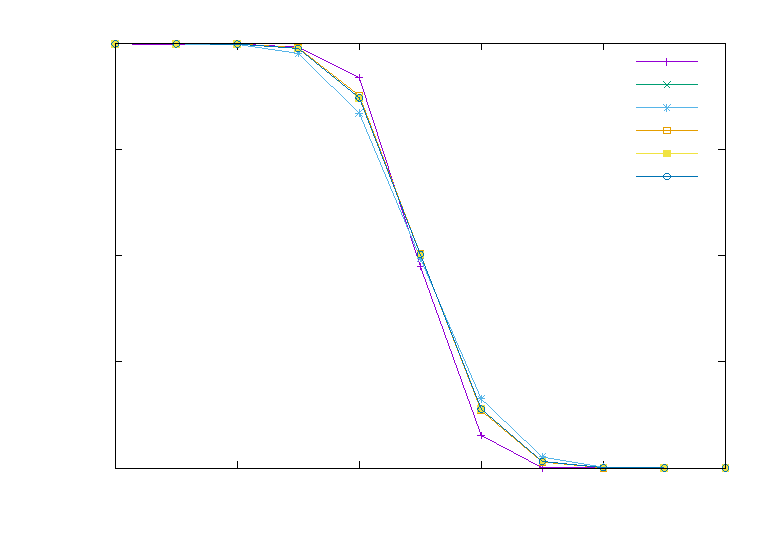
\includegraphics{SmithHutton/1000}}%
    \gplfronttext
  \end{picture}%
\endgroup

	\caption{Distribution of $\phi$ at the output for $\rho/\Gamma=10^{3}$}
	\label{ResSH1000}
\end{figure}
\begin{figure}[h!]
	\centering
	% GNUPLOT: LaTeX picture with Postscript
\begingroup
  \makeatletter
  \providecommand\color[2][]{%
    \GenericError{(gnuplot) \space\space\space\@spaces}{%
      Package color not loaded in conjunction with
      terminal option `colourtext'%
    }{See the gnuplot documentation for explanation.%
    }{Either use 'blacktext' in gnuplot or load the package
      color.sty in LaTeX.}%
    \renewcommand\color[2][]{}%
  }%
  \providecommand\includegraphics[2][]{%
    \GenericError{(gnuplot) \space\space\space\@spaces}{%
      Package graphicx or graphics not loaded%
    }{See the gnuplot documentation for explanation.%
    }{The gnuplot epslatex terminal needs graphicx.sty or graphics.sty.}%
    \renewcommand\includegraphics[2][]{}%
  }%
  \providecommand\rotatebox[2]{#2}%
  \@ifundefined{ifGPcolor}{%
    \newif\ifGPcolor
    \GPcolortrue
  }{}%
  \@ifundefined{ifGPblacktext}{%
    \newif\ifGPblacktext
    \GPblacktexttrue
  }{}%
  % define a \g@addto@macro without @ in the name:
  \let\gplgaddtomacro\g@addto@macro
  % define empty templates for all commands taking text:
  \gdef\gplbacktext{}%
  \gdef\gplfronttext{}%
  \makeatother
  \ifGPblacktext
    % no textcolor at all
    \def\colorrgb#1{}%
    \def\colorgray#1{}%
  \else
    % gray or color?
    \ifGPcolor
      \def\colorrgb#1{\color[rgb]{#1}}%
      \def\colorgray#1{\color[gray]{#1}}%
      \expandafter\def\csname LTw\endcsname{\color{white}}%
      \expandafter\def\csname LTb\endcsname{\color{black}}%
      \expandafter\def\csname LTa\endcsname{\color{black}}%
      \expandafter\def\csname LT0\endcsname{\color[rgb]{1,0,0}}%
      \expandafter\def\csname LT1\endcsname{\color[rgb]{0,1,0}}%
      \expandafter\def\csname LT2\endcsname{\color[rgb]{0,0,1}}%
      \expandafter\def\csname LT3\endcsname{\color[rgb]{1,0,1}}%
      \expandafter\def\csname LT4\endcsname{\color[rgb]{0,1,1}}%
      \expandafter\def\csname LT5\endcsname{\color[rgb]{1,1,0}}%
      \expandafter\def\csname LT6\endcsname{\color[rgb]{0,0,0}}%
      \expandafter\def\csname LT7\endcsname{\color[rgb]{1,0.3,0}}%
      \expandafter\def\csname LT8\endcsname{\color[rgb]{0.5,0.5,0.5}}%
    \else
      % gray
      \def\colorrgb#1{\color{black}}%
      \def\colorgray#1{\color[gray]{#1}}%
      \expandafter\def\csname LTw\endcsname{\color{white}}%
      \expandafter\def\csname LTb\endcsname{\color{black}}%
      \expandafter\def\csname LTa\endcsname{\color{black}}%
      \expandafter\def\csname LT0\endcsname{\color{black}}%
      \expandafter\def\csname LT1\endcsname{\color{black}}%
      \expandafter\def\csname LT2\endcsname{\color{black}}%
      \expandafter\def\csname LT3\endcsname{\color{black}}%
      \expandafter\def\csname LT4\endcsname{\color{black}}%
      \expandafter\def\csname LT5\endcsname{\color{black}}%
      \expandafter\def\csname LT6\endcsname{\color{black}}%
      \expandafter\def\csname LT7\endcsname{\color{black}}%
      \expandafter\def\csname LT8\endcsname{\color{black}}%
    \fi
  \fi
    \setlength{\unitlength}{0.0500bp}%
    \ifx\gptboxheight\undefined%
      \newlength{\gptboxheight}%
      \newlength{\gptboxwidth}%
      \newsavebox{\gptboxtext}%
    \fi%
    \setlength{\fboxrule}{0.5pt}%
    \setlength{\fboxsep}{1pt}%
\begin{picture}(7200.00,5040.00)%
    \gplgaddtomacro\gplbacktext{%
      \csname LTb\endcsname%
      \put(814,704){\makebox(0,0)[r]{\strut{}$0$}}%
      \put(814,1722){\makebox(0,0)[r]{\strut{}$0.5$}}%
      \put(814,2740){\makebox(0,0)[r]{\strut{}$1$}}%
      \put(814,3757){\makebox(0,0)[r]{\strut{}$1.5$}}%
      \put(814,4775){\makebox(0,0)[r]{\strut{}$2$}}%
      \put(946,484){\makebox(0,0){\strut{}$0$}}%
      \put(2117,484){\makebox(0,0){\strut{}$0.2$}}%
      \put(3289,484){\makebox(0,0){\strut{}$0.4$}}%
      \put(4460,484){\makebox(0,0){\strut{}$0.6$}}%
      \put(5632,484){\makebox(0,0){\strut{}$0.8$}}%
      \put(6803,484){\makebox(0,0){\strut{}$1$}}%
    }%
    \gplgaddtomacro\gplfronttext{%
      \csname LTb\endcsname%
      \put(176,2739){\rotatebox{-270}{\makebox(0,0){\strut{}$\phi$}}}%
      \put(3874,154){\makebox(0,0){\strut{}x-position}}%
      \csname LTb\endcsname%
      \put(5816,4602){\makebox(0,0)[r]{\strut{}Reference}}%
      \csname LTb\endcsname%
      \put(5816,4382){\makebox(0,0)[r]{\strut{}CDS}}%
      \csname LTb\endcsname%
      \put(5816,4162){\makebox(0,0)[r]{\strut{}UDS}}%
      \csname LTb\endcsname%
      \put(5816,3942){\makebox(0,0)[r]{\strut{}HDS}}%
      \csname LTb\endcsname%
      \put(5816,3722){\makebox(0,0)[r]{\strut{}PLDS}}%
      \csname LTb\endcsname%
      \put(5816,3502){\makebox(0,0)[r]{\strut{}EDS}}%
    }%
    \gplbacktext
    \put(0,0){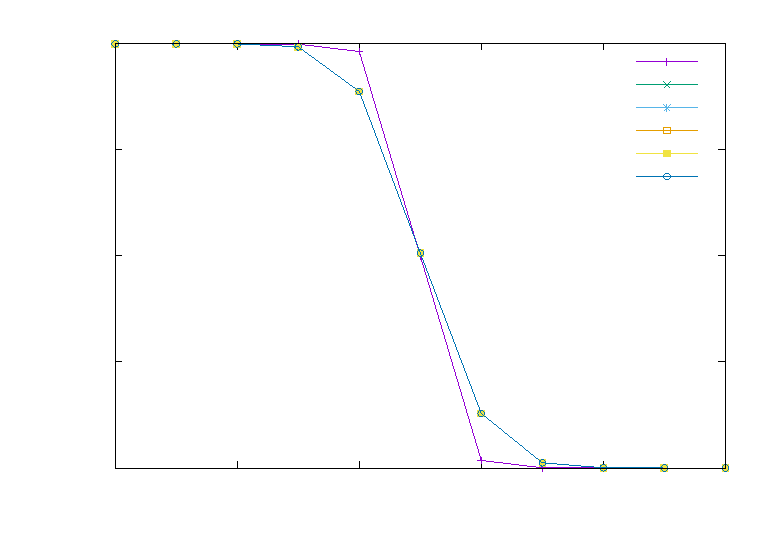
\includegraphics{SmithHutton/1000000}}%
    \gplfronttext
  \end{picture}%
\endgroup

	\caption{Distribution of $\phi$ at the output for $\rho/\Gamma=10^{6}$}
	\label{ResSH1000000}
\end{figure}
It is important to notice that in the cases $\rho/\Gamma=10^{3}$ and $\rho/\Gamma=10^{6}$ CDS diverges, and no results are obtained with this method.

Regarding the behaviour of $\phi$, for low Péclet numbers, its variation its almost linear, but for high Péclets, it becomes more abrupt, almost a vertical line.

Finally, it is interesting to study the variation of the variable $\phi$ in the whole domain. As it is represented in figure \ref{ResuSH10}, for a low Péclet number, since the main transport method is diffusion the variable changes gradually over the domain. But as it increases (figures \ref{ResuSH1000} and \ref{ResuSH1000000}), the change is more abrupt, and there is almost no variation except for the centre bottom zone. The distribution of $\phi$ becomes more symmetrical as the Péclet number increases.

\begin{figure}[h]
	\centering
	% GNUPLOT: LaTeX picture with Postscript
\begingroup
  \makeatletter
  \providecommand\color[2][]{%
    \GenericError{(gnuplot) \space\space\space\@spaces}{%
      Package color not loaded in conjunction with
      terminal option `colourtext'%
    }{See the gnuplot documentation for explanation.%
    }{Either use 'blacktext' in gnuplot or load the package
      color.sty in LaTeX.}%
    \renewcommand\color[2][]{}%
  }%
  \providecommand\includegraphics[2][]{%
    \GenericError{(gnuplot) \space\space\space\@spaces}{%
      Package graphicx or graphics not loaded%
    }{See the gnuplot documentation for explanation.%
    }{The gnuplot epslatex terminal needs graphicx.sty or graphics.sty.}%
    \renewcommand\includegraphics[2][]{}%
  }%
  \providecommand\rotatebox[2]{#2}%
  \@ifundefined{ifGPcolor}{%
    \newif\ifGPcolor
    \GPcolortrue
  }{}%
  \@ifundefined{ifGPblacktext}{%
    \newif\ifGPblacktext
    \GPblacktexttrue
  }{}%
  % define a \g@addto@macro without @ in the name:
  \let\gplgaddtomacro\g@addto@macro
  % define empty templates for all commands taking text:
  \gdef\gplbacktext{}%
  \gdef\gplfronttext{}%
  \makeatother
  \ifGPblacktext
    % no textcolor at all
    \def\colorrgb#1{}%
    \def\colorgray#1{}%
  \else
    % gray or color?
    \ifGPcolor
      \def\colorrgb#1{\color[rgb]{#1}}%
      \def\colorgray#1{\color[gray]{#1}}%
      \expandafter\def\csname LTw\endcsname{\color{white}}%
      \expandafter\def\csname LTb\endcsname{\color{black}}%
      \expandafter\def\csname LTa\endcsname{\color{black}}%
      \expandafter\def\csname LT0\endcsname{\color[rgb]{1,0,0}}%
      \expandafter\def\csname LT1\endcsname{\color[rgb]{0,1,0}}%
      \expandafter\def\csname LT2\endcsname{\color[rgb]{0,0,1}}%
      \expandafter\def\csname LT3\endcsname{\color[rgb]{1,0,1}}%
      \expandafter\def\csname LT4\endcsname{\color[rgb]{0,1,1}}%
      \expandafter\def\csname LT5\endcsname{\color[rgb]{1,1,0}}%
      \expandafter\def\csname LT6\endcsname{\color[rgb]{0,0,0}}%
      \expandafter\def\csname LT7\endcsname{\color[rgb]{1,0.3,0}}%
      \expandafter\def\csname LT8\endcsname{\color[rgb]{0.5,0.5,0.5}}%
    \else
      % gray
      \def\colorrgb#1{\color{black}}%
      \def\colorgray#1{\color[gray]{#1}}%
      \expandafter\def\csname LTw\endcsname{\color{white}}%
      \expandafter\def\csname LTb\endcsname{\color{black}}%
      \expandafter\def\csname LTa\endcsname{\color{black}}%
      \expandafter\def\csname LT0\endcsname{\color{black}}%
      \expandafter\def\csname LT1\endcsname{\color{black}}%
      \expandafter\def\csname LT2\endcsname{\color{black}}%
      \expandafter\def\csname LT3\endcsname{\color{black}}%
      \expandafter\def\csname LT4\endcsname{\color{black}}%
      \expandafter\def\csname LT5\endcsname{\color{black}}%
      \expandafter\def\csname LT6\endcsname{\color{black}}%
      \expandafter\def\csname LT7\endcsname{\color{black}}%
      \expandafter\def\csname LT8\endcsname{\color{black}}%
    \fi
  \fi
    \setlength{\unitlength}{0.0500bp}%
    \ifx\gptboxheight\undefined%
      \newlength{\gptboxheight}%
      \newlength{\gptboxwidth}%
      \newsavebox{\gptboxtext}%
    \fi%
    \setlength{\fboxrule}{0.5pt}%
    \setlength{\fboxsep}{1pt}%
\begin{picture}(7200.00,5040.00)%
    \gplgaddtomacro\gplbacktext{%
    }%
    \gplgaddtomacro\gplfronttext{%
      \csname LTb\endcsname%
      \put(5346,4149){\makebox(0,0)[r]{\strut{}'R10.dat' using 1:2:3}}%
      \csname LTb\endcsname%
      \put(936,624){\makebox(0,0){\strut{}$-1$}}%
      \put(2268,624){\makebox(0,0){\strut{}$-0.5$}}%
      \put(3600,624){\makebox(0,0){\strut{}$0$}}%
      \put(4932,624){\makebox(0,0){\strut{}$0.5$}}%
      \put(6264,624){\makebox(0,0){\strut{}$1$}}%
      \put(748,938){\makebox(0,0)[r]{\strut{}$0$}}%
      \put(748,1615){\makebox(0,0)[r]{\strut{}$0.2$}}%
      \put(748,2292){\makebox(0,0)[r]{\strut{}$0.4$}}%
      \put(748,2968){\makebox(0,0)[r]{\strut{}$0.6$}}%
      \put(748,3645){\makebox(0,0)[r]{\strut{}$0.8$}}%
      \put(748,4322){\makebox(0,0)[r]{\strut{}$1$}}%
      \put(6796,938){\makebox(0,0)[l]{\strut{}$0$}}%
      \put(6796,1276){\makebox(0,0)[l]{\strut{}$0.2$}}%
      \put(6796,1614){\makebox(0,0)[l]{\strut{}$0.4$}}%
      \put(6796,1953){\makebox(0,0)[l]{\strut{}$0.6$}}%
      \put(6796,2291){\makebox(0,0)[l]{\strut{}$0.8$}}%
      \put(6796,2630){\makebox(0,0)[l]{\strut{}$1$}}%
      \put(6796,2968){\makebox(0,0)[l]{\strut{}$1.2$}}%
      \put(6796,3306){\makebox(0,0)[l]{\strut{}$1.4$}}%
      \put(6796,3645){\makebox(0,0)[l]{\strut{}$1.6$}}%
      \put(6796,3983){\makebox(0,0)[l]{\strut{}$1.8$}}%
      \put(6796,4322){\makebox(0,0)[l]{\strut{}$2$}}%
    }%
    \gplbacktext
    \put(0,0){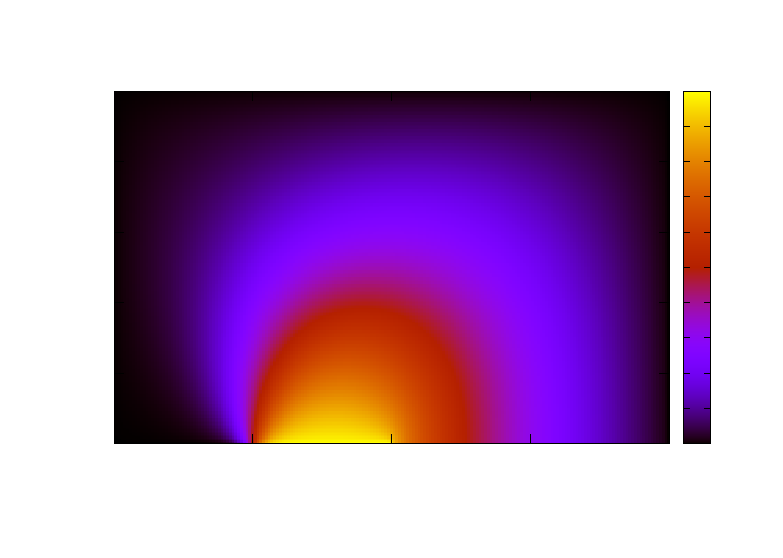
\includegraphics{SmithHutton/UDS/R10}}%
    \gplfronttext
  \end{picture}%
\endgroup

	\caption{Representation of the whole domain for $\rho/\Gamma=10$ (UDS)}
	\label{ResuSH10}
\end{figure}
\begin{figure}[h!]
	\centering
	% GNUPLOT: LaTeX picture with Postscript
\begingroup
  \makeatletter
  \providecommand\color[2][]{%
    \GenericError{(gnuplot) \space\space\space\@spaces}{%
      Package color not loaded in conjunction with
      terminal option `colourtext'%
    }{See the gnuplot documentation for explanation.%
    }{Either use 'blacktext' in gnuplot or load the package
      color.sty in LaTeX.}%
    \renewcommand\color[2][]{}%
  }%
  \providecommand\includegraphics[2][]{%
    \GenericError{(gnuplot) \space\space\space\@spaces}{%
      Package graphicx or graphics not loaded%
    }{See the gnuplot documentation for explanation.%
    }{The gnuplot epslatex terminal needs graphicx.sty or graphics.sty.}%
    \renewcommand\includegraphics[2][]{}%
  }%
  \providecommand\rotatebox[2]{#2}%
  \@ifundefined{ifGPcolor}{%
    \newif\ifGPcolor
    \GPcolortrue
  }{}%
  \@ifundefined{ifGPblacktext}{%
    \newif\ifGPblacktext
    \GPblacktexttrue
  }{}%
  % define a \g@addto@macro without @ in the name:
  \let\gplgaddtomacro\g@addto@macro
  % define empty templates for all commands taking text:
  \gdef\gplbacktext{}%
  \gdef\gplfronttext{}%
  \makeatother
  \ifGPblacktext
    % no textcolor at all
    \def\colorrgb#1{}%
    \def\colorgray#1{}%
  \else
    % gray or color?
    \ifGPcolor
      \def\colorrgb#1{\color[rgb]{#1}}%
      \def\colorgray#1{\color[gray]{#1}}%
      \expandafter\def\csname LTw\endcsname{\color{white}}%
      \expandafter\def\csname LTb\endcsname{\color{black}}%
      \expandafter\def\csname LTa\endcsname{\color{black}}%
      \expandafter\def\csname LT0\endcsname{\color[rgb]{1,0,0}}%
      \expandafter\def\csname LT1\endcsname{\color[rgb]{0,1,0}}%
      \expandafter\def\csname LT2\endcsname{\color[rgb]{0,0,1}}%
      \expandafter\def\csname LT3\endcsname{\color[rgb]{1,0,1}}%
      \expandafter\def\csname LT4\endcsname{\color[rgb]{0,1,1}}%
      \expandafter\def\csname LT5\endcsname{\color[rgb]{1,1,0}}%
      \expandafter\def\csname LT6\endcsname{\color[rgb]{0,0,0}}%
      \expandafter\def\csname LT7\endcsname{\color[rgb]{1,0.3,0}}%
      \expandafter\def\csname LT8\endcsname{\color[rgb]{0.5,0.5,0.5}}%
    \else
      % gray
      \def\colorrgb#1{\color{black}}%
      \def\colorgray#1{\color[gray]{#1}}%
      \expandafter\def\csname LTw\endcsname{\color{white}}%
      \expandafter\def\csname LTb\endcsname{\color{black}}%
      \expandafter\def\csname LTa\endcsname{\color{black}}%
      \expandafter\def\csname LT0\endcsname{\color{black}}%
      \expandafter\def\csname LT1\endcsname{\color{black}}%
      \expandafter\def\csname LT2\endcsname{\color{black}}%
      \expandafter\def\csname LT3\endcsname{\color{black}}%
      \expandafter\def\csname LT4\endcsname{\color{black}}%
      \expandafter\def\csname LT5\endcsname{\color{black}}%
      \expandafter\def\csname LT6\endcsname{\color{black}}%
      \expandafter\def\csname LT7\endcsname{\color{black}}%
      \expandafter\def\csname LT8\endcsname{\color{black}}%
    \fi
  \fi
    \setlength{\unitlength}{0.0500bp}%
    \ifx\gptboxheight\undefined%
      \newlength{\gptboxheight}%
      \newlength{\gptboxwidth}%
      \newsavebox{\gptboxtext}%
    \fi%
    \setlength{\fboxrule}{0.5pt}%
    \setlength{\fboxsep}{1pt}%
\begin{picture}(7200.00,5040.00)%
    \gplgaddtomacro\gplbacktext{%
    }%
    \gplgaddtomacro\gplfronttext{%
      \csname LTb\endcsname%
      \put(5346,4149){\makebox(0,0)[r]{\strut{}'R1000.dat' using 1:2:3}}%
      \csname LTb\endcsname%
      \put(936,624){\makebox(0,0){\strut{}$-1$}}%
      \put(2268,624){\makebox(0,0){\strut{}$-0.5$}}%
      \put(3600,624){\makebox(0,0){\strut{}$0$}}%
      \put(4932,624){\makebox(0,0){\strut{}$0.5$}}%
      \put(6264,624){\makebox(0,0){\strut{}$1$}}%
      \put(748,938){\makebox(0,0)[r]{\strut{}$0$}}%
      \put(748,1615){\makebox(0,0)[r]{\strut{}$0.2$}}%
      \put(748,2292){\makebox(0,0)[r]{\strut{}$0.4$}}%
      \put(748,2968){\makebox(0,0)[r]{\strut{}$0.6$}}%
      \put(748,3645){\makebox(0,0)[r]{\strut{}$0.8$}}%
      \put(748,4322){\makebox(0,0)[r]{\strut{}$1$}}%
      \put(6796,938){\makebox(0,0)[l]{\strut{}$0$}}%
      \put(6796,1276){\makebox(0,0)[l]{\strut{}$0.2$}}%
      \put(6796,1614){\makebox(0,0)[l]{\strut{}$0.4$}}%
      \put(6796,1953){\makebox(0,0)[l]{\strut{}$0.6$}}%
      \put(6796,2291){\makebox(0,0)[l]{\strut{}$0.8$}}%
      \put(6796,2630){\makebox(0,0)[l]{\strut{}$1$}}%
      \put(6796,2968){\makebox(0,0)[l]{\strut{}$1.2$}}%
      \put(6796,3306){\makebox(0,0)[l]{\strut{}$1.4$}}%
      \put(6796,3645){\makebox(0,0)[l]{\strut{}$1.6$}}%
      \put(6796,3983){\makebox(0,0)[l]{\strut{}$1.8$}}%
      \put(6796,4322){\makebox(0,0)[l]{\strut{}$2$}}%
    }%
    \gplbacktext
    \put(0,0){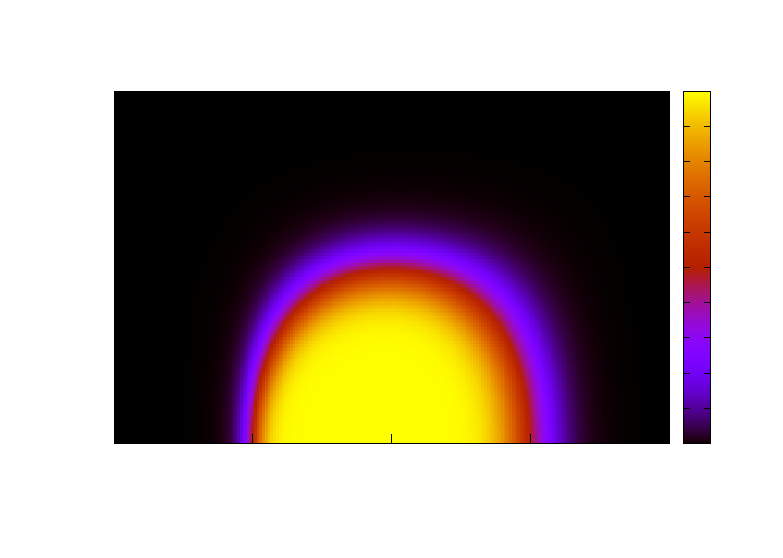
\includegraphics{SmithHutton/UDS/R1000}}%
    \gplfronttext
  \end{picture}%
\endgroup

	\caption{Representation of the whole domain for $\rho/\Gamma=10^{3}$ (UDS)}
	\label{ResuSH1000}
\end{figure}
\begin{figure}[h]
	\centering
	% GNUPLOT: LaTeX picture with Postscript
\begingroup
  \makeatletter
  \providecommand\color[2][]{%
    \GenericError{(gnuplot) \space\space\space\@spaces}{%
      Package color not loaded in conjunction with
      terminal option `colourtext'%
    }{See the gnuplot documentation for explanation.%
    }{Either use 'blacktext' in gnuplot or load the package
      color.sty in LaTeX.}%
    \renewcommand\color[2][]{}%
  }%
  \providecommand\includegraphics[2][]{%
    \GenericError{(gnuplot) \space\space\space\@spaces}{%
      Package graphicx or graphics not loaded%
    }{See the gnuplot documentation for explanation.%
    }{The gnuplot epslatex terminal needs graphicx.sty or graphics.sty.}%
    \renewcommand\includegraphics[2][]{}%
  }%
  \providecommand\rotatebox[2]{#2}%
  \@ifundefined{ifGPcolor}{%
    \newif\ifGPcolor
    \GPcolortrue
  }{}%
  \@ifundefined{ifGPblacktext}{%
    \newif\ifGPblacktext
    \GPblacktexttrue
  }{}%
  % define a \g@addto@macro without @ in the name:
  \let\gplgaddtomacro\g@addto@macro
  % define empty templates for all commands taking text:
  \gdef\gplbacktext{}%
  \gdef\gplfronttext{}%
  \makeatother
  \ifGPblacktext
    % no textcolor at all
    \def\colorrgb#1{}%
    \def\colorgray#1{}%
  \else
    % gray or color?
    \ifGPcolor
      \def\colorrgb#1{\color[rgb]{#1}}%
      \def\colorgray#1{\color[gray]{#1}}%
      \expandafter\def\csname LTw\endcsname{\color{white}}%
      \expandafter\def\csname LTb\endcsname{\color{black}}%
      \expandafter\def\csname LTa\endcsname{\color{black}}%
      \expandafter\def\csname LT0\endcsname{\color[rgb]{1,0,0}}%
      \expandafter\def\csname LT1\endcsname{\color[rgb]{0,1,0}}%
      \expandafter\def\csname LT2\endcsname{\color[rgb]{0,0,1}}%
      \expandafter\def\csname LT3\endcsname{\color[rgb]{1,0,1}}%
      \expandafter\def\csname LT4\endcsname{\color[rgb]{0,1,1}}%
      \expandafter\def\csname LT5\endcsname{\color[rgb]{1,1,0}}%
      \expandafter\def\csname LT6\endcsname{\color[rgb]{0,0,0}}%
      \expandafter\def\csname LT7\endcsname{\color[rgb]{1,0.3,0}}%
      \expandafter\def\csname LT8\endcsname{\color[rgb]{0.5,0.5,0.5}}%
    \else
      % gray
      \def\colorrgb#1{\color{black}}%
      \def\colorgray#1{\color[gray]{#1}}%
      \expandafter\def\csname LTw\endcsname{\color{white}}%
      \expandafter\def\csname LTb\endcsname{\color{black}}%
      \expandafter\def\csname LTa\endcsname{\color{black}}%
      \expandafter\def\csname LT0\endcsname{\color{black}}%
      \expandafter\def\csname LT1\endcsname{\color{black}}%
      \expandafter\def\csname LT2\endcsname{\color{black}}%
      \expandafter\def\csname LT3\endcsname{\color{black}}%
      \expandafter\def\csname LT4\endcsname{\color{black}}%
      \expandafter\def\csname LT5\endcsname{\color{black}}%
      \expandafter\def\csname LT6\endcsname{\color{black}}%
      \expandafter\def\csname LT7\endcsname{\color{black}}%
      \expandafter\def\csname LT8\endcsname{\color{black}}%
    \fi
  \fi
    \setlength{\unitlength}{0.0500bp}%
    \ifx\gptboxheight\undefined%
      \newlength{\gptboxheight}%
      \newlength{\gptboxwidth}%
      \newsavebox{\gptboxtext}%
    \fi%
    \setlength{\fboxrule}{0.5pt}%
    \setlength{\fboxsep}{1pt}%
\begin{picture}(7200.00,5040.00)%
    \gplgaddtomacro\gplbacktext{%
    }%
    \gplgaddtomacro\gplfronttext{%
      \csname LTb\endcsname%
      \put(5346,4149){\makebox(0,0)[r]{\strut{}'R1000000.dat' using 1:2:3}}%
      \csname LTb\endcsname%
      \put(936,624){\makebox(0,0){\strut{}$-1$}}%
      \put(2268,624){\makebox(0,0){\strut{}$-0.5$}}%
      \put(3600,624){\makebox(0,0){\strut{}$0$}}%
      \put(4932,624){\makebox(0,0){\strut{}$0.5$}}%
      \put(6264,624){\makebox(0,0){\strut{}$1$}}%
      \put(748,938){\makebox(0,0)[r]{\strut{}$0$}}%
      \put(748,1615){\makebox(0,0)[r]{\strut{}$0.2$}}%
      \put(748,2292){\makebox(0,0)[r]{\strut{}$0.4$}}%
      \put(748,2968){\makebox(0,0)[r]{\strut{}$0.6$}}%
      \put(748,3645){\makebox(0,0)[r]{\strut{}$0.8$}}%
      \put(748,4322){\makebox(0,0)[r]{\strut{}$1$}}%
      \put(6796,938){\makebox(0,0)[l]{\strut{}$0$}}%
      \put(6796,1276){\makebox(0,0)[l]{\strut{}$0.2$}}%
      \put(6796,1614){\makebox(0,0)[l]{\strut{}$0.4$}}%
      \put(6796,1953){\makebox(0,0)[l]{\strut{}$0.6$}}%
      \put(6796,2291){\makebox(0,0)[l]{\strut{}$0.8$}}%
      \put(6796,2630){\makebox(0,0)[l]{\strut{}$1$}}%
      \put(6796,2968){\makebox(0,0)[l]{\strut{}$1.2$}}%
      \put(6796,3306){\makebox(0,0)[l]{\strut{}$1.4$}}%
      \put(6796,3645){\makebox(0,0)[l]{\strut{}$1.6$}}%
      \put(6796,3983){\makebox(0,0)[l]{\strut{}$1.8$}}%
      \put(6796,4322){\makebox(0,0)[l]{\strut{}$2$}}%
    }%
    \gplbacktext
    \put(0,0){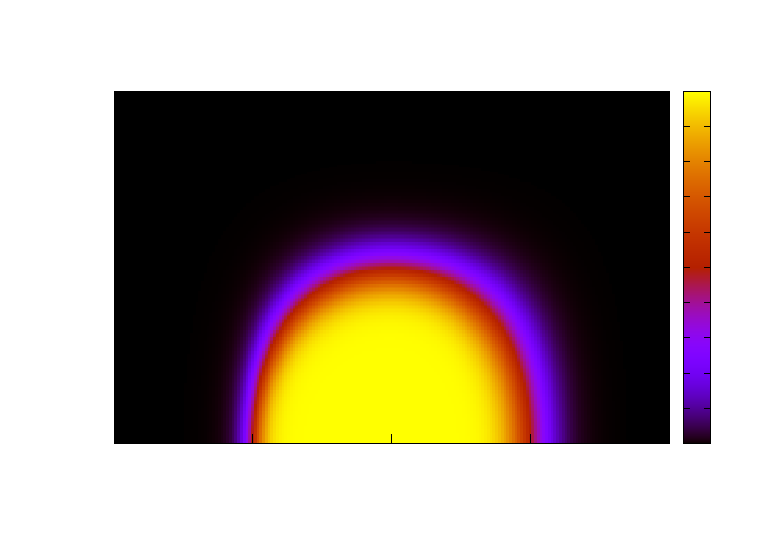
\includegraphics{SmithHutton/UDS/R1000000}}%
    \gplfronttext
  \end{picture}%
\endgroup

	\caption{Representation of the whole domain for $\rho/\Gamma=10^{6}$ (UDS)}
	\label{ResuSH1000000}
\end{figure}

As a conclusion, it can be stated that for low Péclet numbers, diffusion dominates over advection, and it tends to uniformly distribute the properties of the inlet to the whole domain. However, as the Péclet number increases advection becomes more important, the influence of the inlet decreases and the velocity field is the one that determines the distribution of the variable $\phi$.

Some of the results are plotted in this section, but due to the amount of information, not all of them are in the report. To see more results refer to Attachment A.